\section{Architecture Overview}
\begin{figure}[ht]
\centering
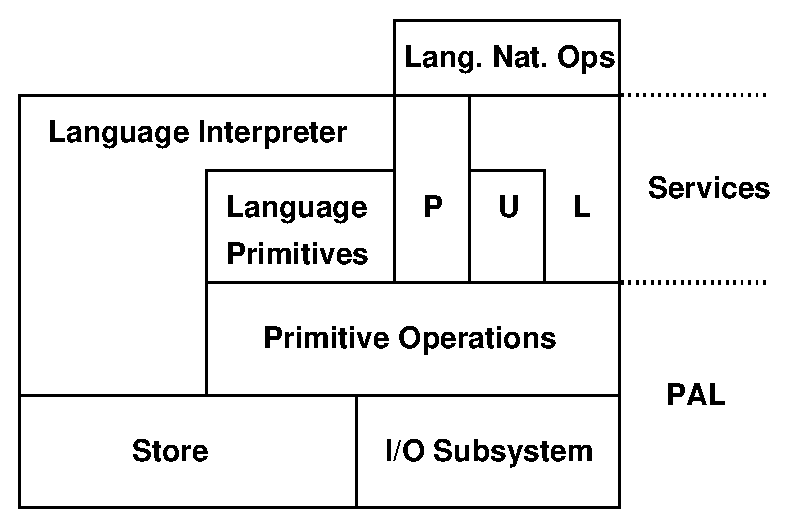
\includegraphics[width=6cm]{figures/architecture.eps}
\caption{\label{vm_architecture} {\it VM Architecture}}
\end{figure}
Figure \ref{vm_architecture} shows the architecture of the virtual
machine as a layered block diagram.
The architecture is organized into three layers, namely
the platform abstraction layer (PAL),
the service layer and finally one or more co-existing
language layers.
\begin{paragraph}{Platform abstraction layer.}
This layer abstracts away the details of the underlying platform
by providing an abstract store and generic IO support.

Every datastructure of the machine including both code and data
is stored into the store. The store provides for automatic garbage collection.

In addion, this layer provides some primitive datatypes
containing some core data structures.
\end{paragraph}
\begin{paragraph}{System service layer.}
A central service for a open programing system is the availability
of persistent state and the ability to link modules during runtime.

These services are provided with the Unpickler (U), Pickler (P) and linker (L).

This layer is generic for all languages. Idea:
have mapping on blocks. Describe mapping during export.
Apply platform specific mapping during import.
\end{paragraph}
\begin{paragraph}{Language specific layers.}
Each layer is composed of four parts:
\begin{enumerate}
\item Language specific data layer (LDL)
\item Language specific primitives
\item Language specific native operations
\item One or more language interpreter
\end{enumerate}
The {\em LDL} maps the language specific data structures to store data
structures. If two languages have intersections within their LDL, they
can interop on data structure level on this intersection.

Most language api are based on a set of primitives which operate
on the language datastructures.
Therefore, the machines supports language specific primitives.

Each language needs to introduce at least one interpreter to
execute its tasks. The language layer also introduces the
code representation of the language.
\end{paragraph}
